\documentclass[11pt]{article}

\usepackage[margin=1in,includefoot]{geometry}
\usepackage{fancyhdr}
\usepackage[colorlinks=true,urlcolor=blue,citecolor=blue]{hyperref}
\usepackage{url}
\usepackage{graphicx}
\usepackage{listings}
\pagestyle{fancy}
\renewcommand\footrulewidth{1pt}
\makeatletter
\g@addto@macro{\UrlBreaks}{\UrlOrds}
\makeatother
\lstset{
   basicstyle=\fontsize{6}{10}\selectfont\ttfamily
}

\begin{document}

\begin{titlepage}

	\begin{center}
	
	\huge ITCS443 Parallel and Distributed Systems\\
	[0.8cm]
	\LARGE Project Report\\
	[0.3cm]
	\Large Hadoop - Calculate Success Rate of the Advertisements on Facebook\\
	[1.5cm]
	\LARGE Members\\
	[0.5cm]
	\Large Kasidit   	Ruaydee   		   5988117\\
	[0.2cm]
	\Large Pasin        Pubpateeravanich   5988186\\
	[0.2cm] 
	\Large Patthanayu   Rueangdej   	   5988195\\ 
	[0.2cm]
	\Large Nuwat   		Tantbirojn   	   5988240\\    
	[1.5cm]
	\LARGE Presented to\\
	[0.2cm]
	\Large Dr. Putt Sakdhnagool\\
	[1.5cm]
	\Large Faculty of Information and Communication Technology\\
	[0.2cm]
	\Large Mahidol University\\
	[0.2cm]
	\Large 2018
	\begin{figure}[h]
	\centering
	
\includegraphics[scale=0.35]{mu}
	\end{figure}
	
	\end{center}
	
\end{titlepage}

\section{Introduction}\label{sec:intro}
\subsection{Project goal}
To successfully created a project using Hadoop to analyze big data and able to give the correct and accurate output.
\subsection{Why is this project interesting / worth to do?}
From the lecture class and doing the lab, we think that we still don't know much about the whole concept of Hadoop and the way it approach to the big data. For the better understanding, we tried to learn and create a Hadoop project that can work with the datasets we have and able to provide us a good result. If we understand how to implement Hadoop, we could use this knowledge to adapt in many projects that related to analyzing big data in the future.

In this project, we've created a mock datasets of Facebook advertisement success rate and tried to calculate to know that, which type of the advertisement has high or low success rate for each province in Thailand. We got this idea from past project in web programming class, so we tried to adapt it in this project. We've tried to search for the datasets of another topics, but we didn't find one that interest us.


\newpage
\section{Methodology / Algorithm}\label{sec:method}
\subsection{High-level description of the project / algorithm}
In this project, we implement Hadoop project on Ubuntu with Java language. The main function of this project is to calculate the average success rate of advertisement on Facebook in each province in Thailand.

The datasets we used as the input in this project is a mock datasets that we created by ourselves. The name of datasets is "FB.txt". The datasets has information about advertisements that have been displayed on facebook and their success. The datasets consist of 51 list of input data with 7 attributes.

\begin{figure}[h]
\centering
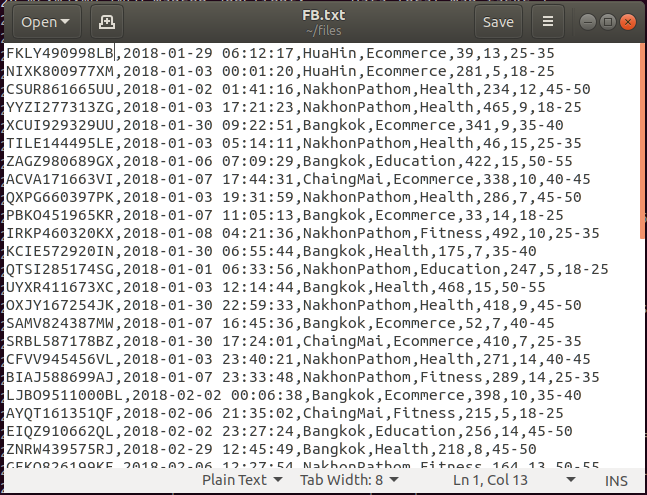
\includegraphics[scale=0.7]{in0}
\caption{Datasets of Facebook advertisement success rate "FB.txt"}
\end{figure}

The first attribute is advertisement ID. The second attribute is the timestamp of advertisement. The third attribute is the province that the advertisement is shown. The forth attribute is the type of the advertisement. The fifth attribute is the amount of click on the advertisement. The sixth attribute is the amount of sell on the advertisement. The last attribute is the age group of the advertisement.

The program will calculate the average success rate of each advertisement in each province by using 4 attributes for calculation, province, type of advertisement, amount of click, and amount of sell. 

For example, there are 3 timestamp of Ecommerce advertisement that is shown in HuaHin. First, a program will calcurates advertisment success rate for each one. Suppose that the first one has amount of click = 39, and amount of sell = 13. The success rate for the first one will be = 13/39*100 = 33.3. 


\newpage
After a program calculated all 3 of the data, the first one is 33.3, the second one is 1.77, and the third one is 30, a program will calculate the average success rate of Ecommerce advertisement in Huahin by combining all 3 success rate and divide by number that the advertisement is shown. The final result will be = (33.3+1.77+30)/3 = 21.69, so the average Ecommerce advertisement success rate in HuaHin will be 21.69. 

\subsection{Detailed explanation of algorithm}
\subsubsection{FacebookMapper.java}
In this class, a program will receive lines of the input from datasets. First, the value will be store in line and split into array of words, which will give us 7 elements. After that, a program will define key value pair that will be use to calculate success rate. Since a program have to calculate success rate of each type of advertisement, so the key will be the forth element of array which is the type of advertisement, and the value will be the combination of third, fifth, and sixth element of array, which are province, amount of click, and amount of sell.\\
[0.5 cm] 

\begin{figure}[h]
\centering
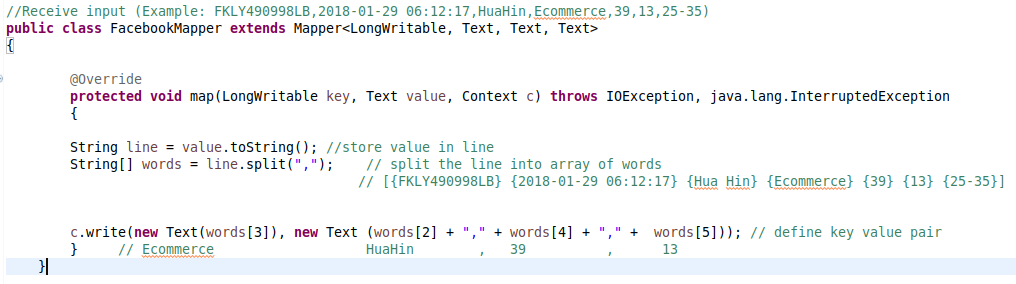
\includegraphics[scale=0.65]{code2}
\caption{Mapper class "FacebookMapper"}
\end{figure}

\newpage


\subsubsection{FacebookReducer.java}
In this class, the map will be reduced and calculate the final result. The reducer class will have two tasks, the first one is calculate success rate and count number, and the second one is calculate the average of success rate of the advertisement. We declared HashMap called "cityDate" to be a storage of key value pair that we get from the task of calculating success rate and count number. A program will get each value in the value list to calculate for each iteration. Suppose a program is calculating for average success rate of the Ecommerce advertisement. \\
[0.5 cm]

\begin{figure}[h]
\centering
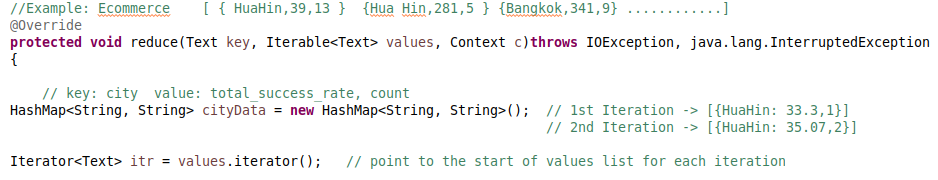
\includegraphics[scale=0.7]{code3}
\caption{HashMap and Iterator}
\end{figure}


\newpage
In the loop, it will be a calculation of success rate and count number. Suppose this is the first iteration. Variable string "f" will be the first element of the value list which is HuaHin,39,13. After that, it will be split into array of 3 elements. Variable string "location" will be province. Variable "clickCount" will be the amount of click. Variable "conversionCount" will be the amount of sell. Since the amount of number and amount of sell are receive as string type, so we have to use "Integer.parseInt()" to convert them to integer for the calculation. Now, we have numbers for calculating the average success rate, which will will store in variable "succRate" by calculating from conversionCount/(clickCount*1.0)*100 and the result will be 33.3. For the first iteration, a program will not enter if-condition since there still no key value pair in the HashMap. In this case, it will go to else statement and put the key as a "location" and values as "succRate", and "1".
Therefore, the first element of HashMap will be [{HuaHin: 33.3,1}].\\[0.5 cm]

\begin{figure}[h]
\centering
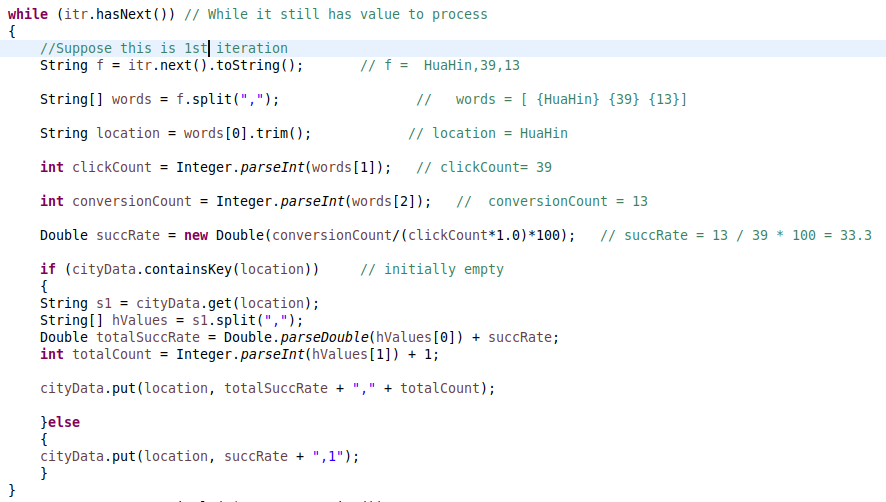
\includegraphics[scale=0.7]{code4}
\caption{1st iteration of calculation in the loop}
\end{figure}

\newpage
In the 2nd iteration, it will be calculation for second element of the value list which is HuaHin,281,5. All of the process will be the same except the if-condition. This time, there is a key value pair in the HashMap which is came from the 1st iteration (HuaHin: 33.3,1). Variable string "s1" will be the value part of HuaHin in HashMap. After that, split the string of 33.3,1 into array of [{33.3} {1}]. Again, we have to convert string to double to do the calculation. Variable "totalSuccrate" will be summation of the success rate. Then, add 1 to count number. The first element which is [{HuaHin:33.3,1}] will be replaced with [{HuaHin:35.07,2}]
[0.5 cm]

\begin{figure}[h]
\centering
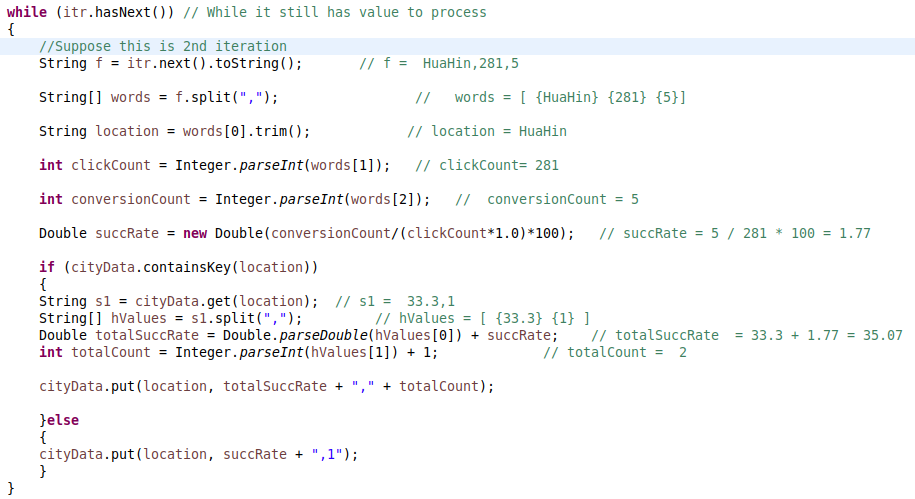
\includegraphics[scale=0.7]{code5}
\caption{2nd iteration of calculation in the loop}
\end{figure}


After the loop is ended, a program will start to calculate for the average of success rate. Suppose the first element of HashMap is [{HuaHin:65.07,3}]. A program will split value into array of 2 elements, and convert them into double for the calculation of success rate average which will be 65.07/3. Finally, the output key will be "Ecommerce", and the value will be "HuaHin" and "21.69"

\begin{figure}[h]
\centering
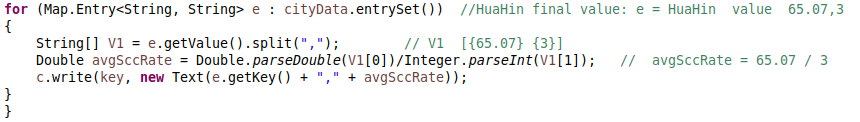
\includegraphics[scale=0.7]{code6}
\caption{Calculation for average success rate}
\end{figure}



\newpage
\section{Experiment and results}\label{sec:exp}
\subsubsection*{Running a program}
To run the program, first we have to export all of 3 classes that we've created into a JAR file. The main class that will be chose to run first is a driver class. In this place, we exported our JAR file name's "Facebook01.jar" at /home/patthanayu/Facebook01.jar. 

\begin{figure}[h]
\centering
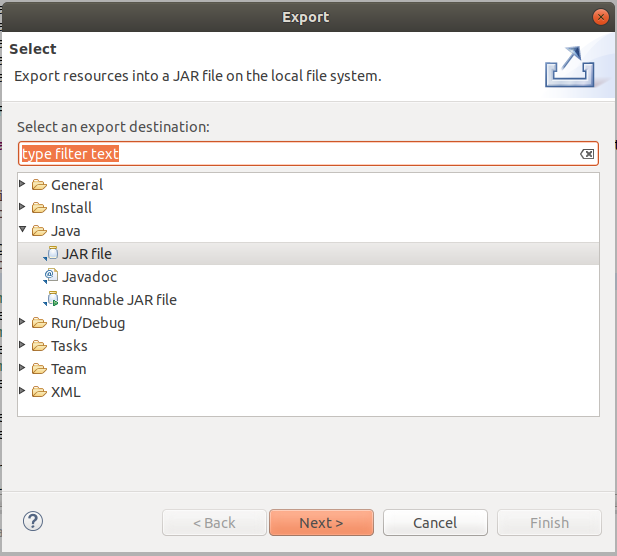
\includegraphics[scale=0.45]{res}
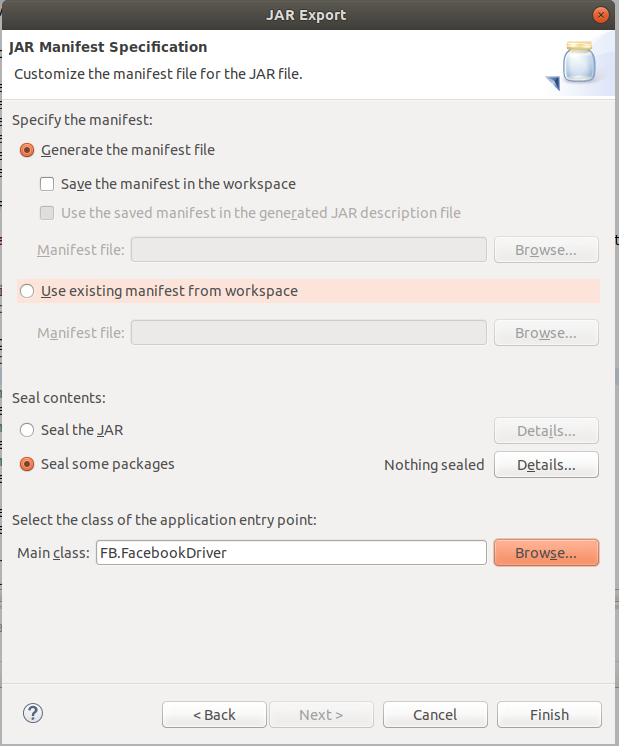
\includegraphics[scale=0.45]{res2}
\caption{Export into a JAR file}
\end{figure}

After Jar file is created, open terminal to start running the code. First, we have to type in the command "ssh localhost". It's like the way to make sure that "localhost" is added to the list of hosts so that script execution doesn't get interrupted by localhost's authenticity trusting question\cite{loc}.

\begin{figure}[h]
\centering
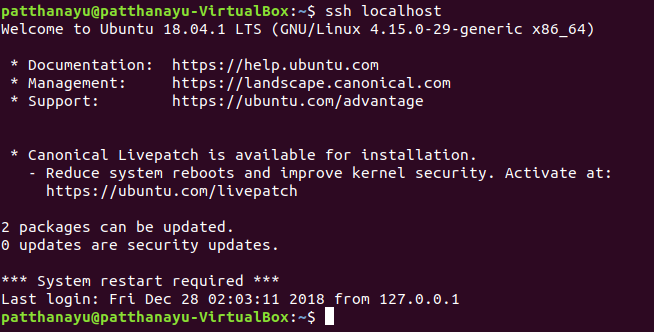
\includegraphics[scale=0.55]{in4}
\caption{Creating connection "ssh localhost"}
\end{figure}


\newpage
After the connection is completed, we will start hadoop process by using "bin/start-all.sh".

\begin{figure}[h]
\centering
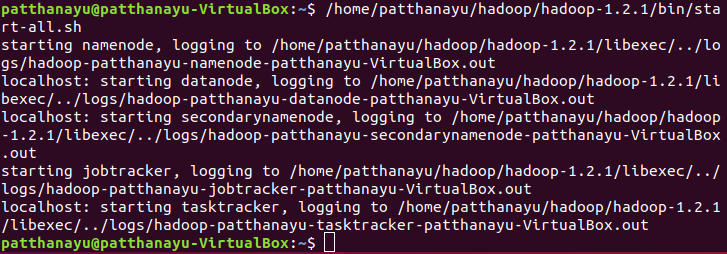
\includegraphics[scale=0.7]{in5}
\caption{Start hadoop "start-all.sh"}
\end{figure}

In this process, we defined the path of the input to be in /user/patthanayu/ which is in HDFS. We can copy the datasets file into HDFS by using the command "bin/hadoop dfs -put /location of input file/  /destination of input file/".

\begin{figure}[h]
\centering
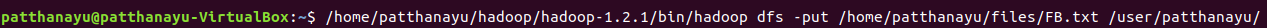
\includegraphics[scale=0.55]{in00}
\caption{Copy datasets file into HDFS}
\end{figure}

\newpage
Now, we can start to run our project by using the command "bin/hadoop jar /home/patthanayu/Facebook01.jar"

\begin{figure}[h]
\centering
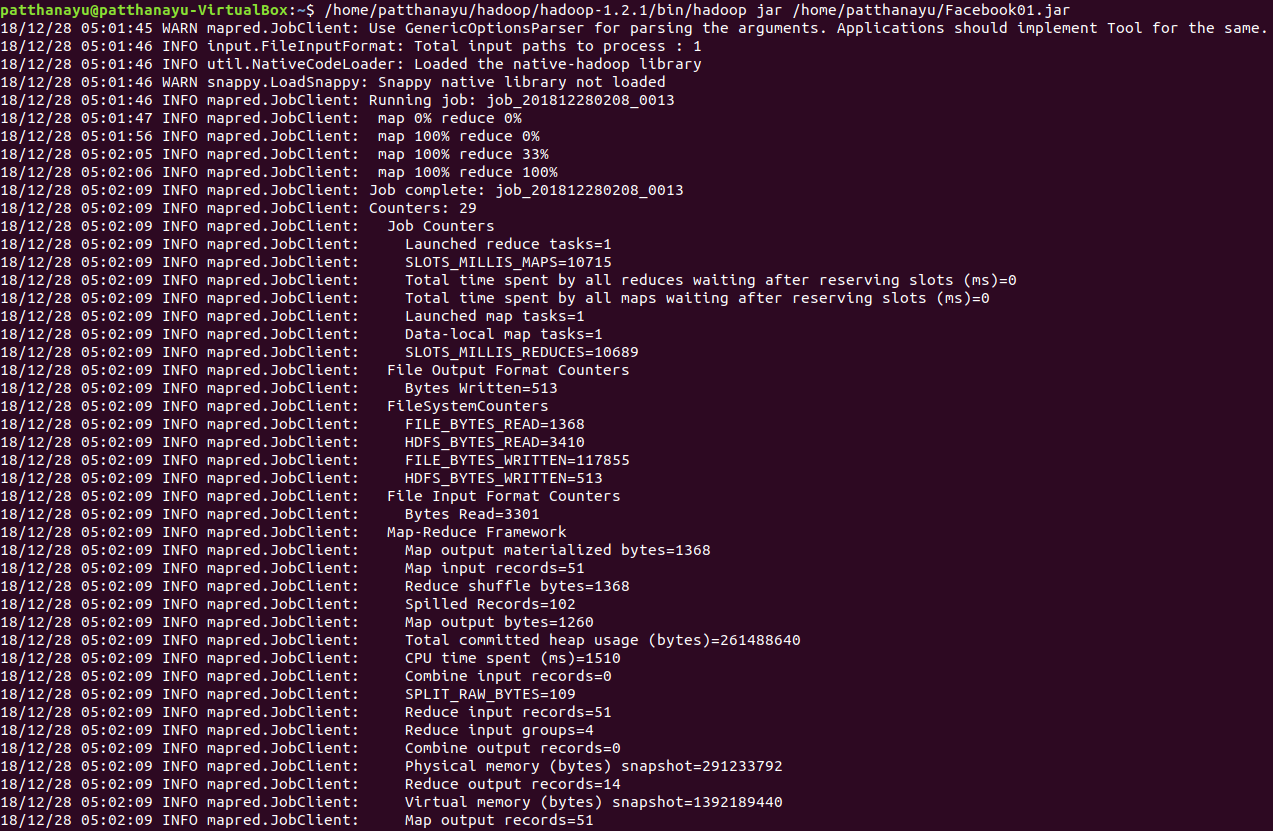
\includegraphics[scale=0.5]{in1}
\caption{Running JAR file}
\end{figure}

There will be files that was generated in /user/patthanayu/Result directory. Use the command "bin/hadoop fs -ls /user/patthanayu/Result"

\begin{figure}[h]
\centering
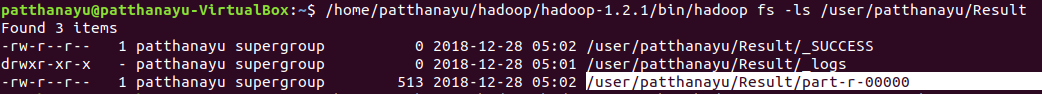
\includegraphics[scale=0.65]{in2}
\caption{3 files in "Result" directory}
\end{figure}


\newpage
To see the result, we use the command "bin/hadoop fs -cat /user/patthanayu/Result/part-r-0000" to copy the output and show. The location of the output can be seen in the directory above, so we can copy and paste (the highlighted part in white). Finally, we will get the result of the project which the average success rate of each advertisement type in each province. The output will consist of 3 columns, type of advertisement, province, and average success rate

\begin{figure}[h]
\centering
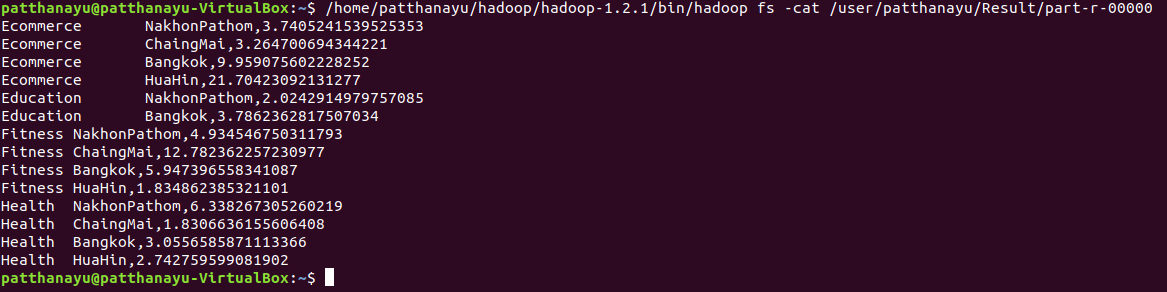
\includegraphics[scale=0.58]{in3}
\caption{The result of the project "Ads type,   Province, and avg success rate"}
\end{figure}

After we've done with running project, we have to stop the hadoop process by using the command "bin/stop-all.sh"

\begin{figure}[h]
\centering
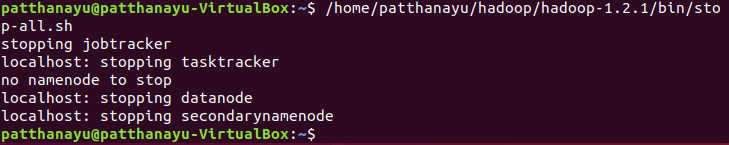
\includegraphics[scale=0.7]{in6}
\caption{Stop using hadoop "stop-all.sh"}
\end{figure}


\newpage
Talking about the result, we tried to check the accuracy of the project output by calculating the output of the datasets manually. This is one of the advantage when we use a small datasets. From the result we get from manually calculation, we will see that when compare with the output from the project, the result is correct and accurate. The list of result will be shown below.\\
- HuaHin,Ecommerce = 21.59\\
- NakhonPathom,Health = 6.338\\
- Bangkok,Ecommerce = 9.959\\
- Bangkok,Education = 3.786\\
- ChaingMai,Ecommerce = 3.25\\
- NakhonPathom,Fitness = 4.934\\
- Bangkok,Health = 3.055\\
- NakhonPathom,Education = 2.024\\
- ChiangMai,Fitness = 12.782\\
- NakhonPathom,Ecommerce = 3.740\\
- HuaHin,Health = 2.742\\
- HuaHin,Fitness = 1.834\\
- ChaingMai,Health = 1.830\\
- Bangkok,Fitness = 5.947

\begin{figure}[h]
\centering
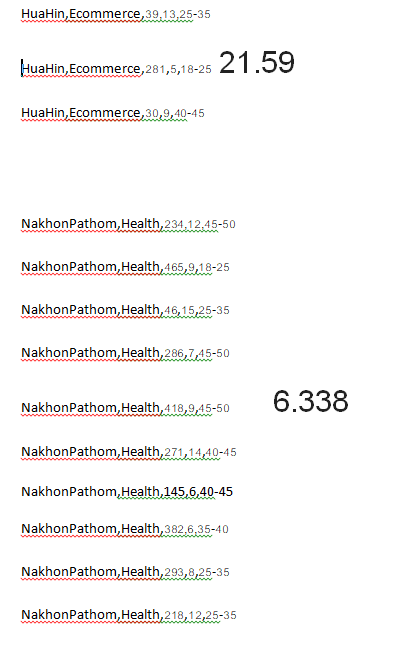
\includegraphics[scale=0.4]{cal1}
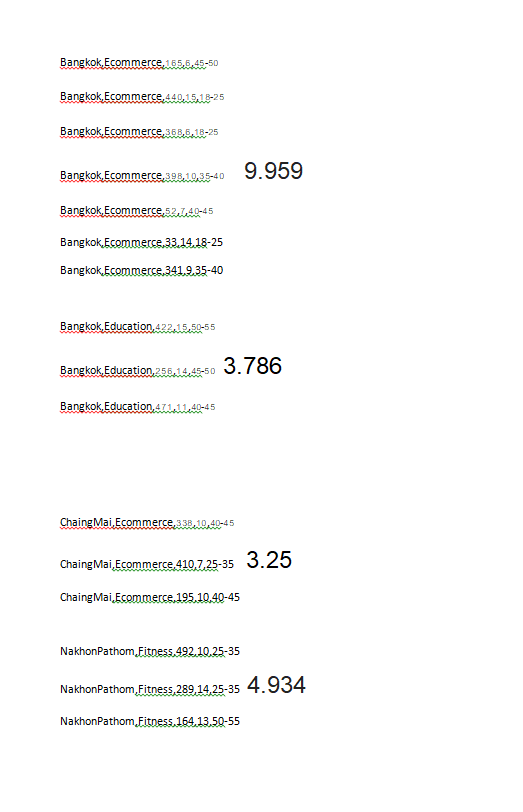
\includegraphics[scale=0.4]{cal2}
\caption{Manual calculation result part 1}
\end{figure}
\newpage
\begin{figure}[h]
\centering
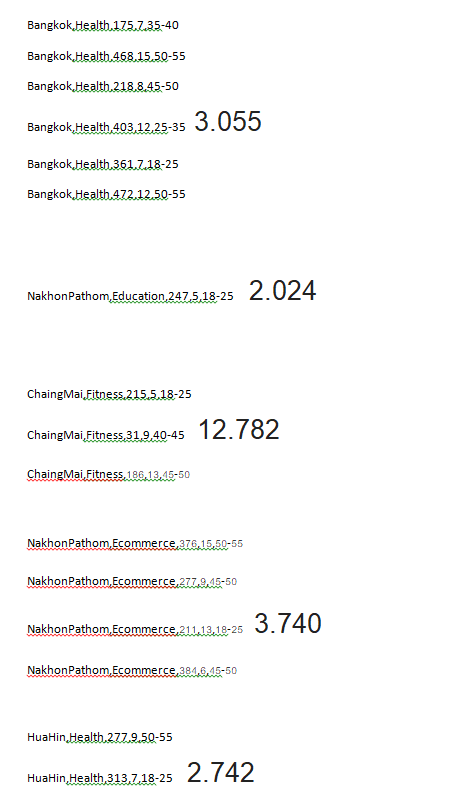
\includegraphics[scale=0.45]{cal3}
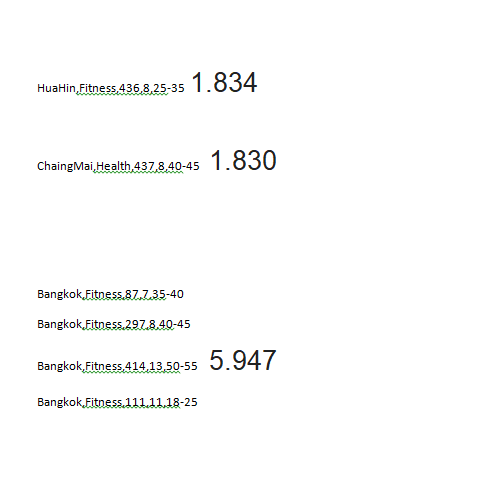
\includegraphics[scale=0.45]{cal4}
\caption{Manual calculation result part 2}
\end{figure}

\newpage
\section{Discussion and conclusion}\label{sec:dis}
\subsection{Discuss the results of your work}
After the discussion about the result, we've found that the project that's created using Hadoop can analyzing the datasets and provide us the accurate and satisfied result. There are reasons we created our own datasets. First of all, it allow us to easily do a manual calculation to give an experiment result. Another reason is that it's easy for us to manage the datasets structure in the project since we create our own. Plus, the time we have is quite short, so we considered to create well-structured datasets with small amount of data.

Another thing that happened in this project is the setup for running Hadoop on virtual machine. We've found many problems, but luckily we able to managed these problem and eventually finished this project. The references of helpful resources for us will be in the references\cite{luc}\cite{mun}\cite{boh}\cite{sau}.
\subsection{How to further improve the work}
If we have more time and opportunity to improve the project, we would use the real datasets that available on the internet which is the real big data, so we able to assure that we can implement Hadoop to analyze big data in the real world.


\newpage
\begin{thebibliography}{9}

\bibitem{loc}
Dean Chen. (2014). \textit{what actually happens when "ssh localhost" command is executed.} [online] Stack Overflow. Available at:
\\\url{https://stackoverflow.com/questions/21926323/what-actually-happens-when-ssh-localhost-command-is-executed}

\bibitem{luc}
lucifer. (2014). \textit{Hadoop command not found.} [online] Stack Overflow. Available at:
\\\url{https://stackoverflow.com/questions/21369102/hadoop-command-not-found?fbclid=IwAR0iH8cZ-0cB5Swmkw4Lb8wkdblzEoJs4_qqVsv1prVuKBbTe8p6d_J1BeM}

\bibitem{mun} 
Munichong.  (2013). \textit{Hadoop: start-dfs.sh permission denied.}  [online] Stack Overflow. Available at: 
\\\url{https://stackoverflow.com/questions/15211848/hadoop-start-dfs-sh-permission-denied}

\bibitem{boh}
Bohn. (2013). \textit{Hadoop is asking for the input path to be on localhost 9000.} Stack Overflow. [online] Available at:
\\\url{https://stackoverflow.com/questions/15732597/hadoop-is-asking-for-the-input-path-to-be-on-localhost-9000/15733487}

\bibitem{sau} 
Saurabh Chhajed. (2014). \textit{Top 10 Hadoop Shell Commands to Manage HDFS - DZone Big Data.} [online] Available at:
\\\url{https://dzone.com/articles/top-10-hadoop-shell-commands}

\end{thebibliography}

\newpage
\section*{Appendix}\label{sec:app}
\subsection*{FacebookMapper.java}
\begin{lstlisting}
package FB;

import java.io.IOException;

import org.apache.hadoop.io.Text;
import org.apache.hadoop.io.LongWritable;
import org.apache.hadoop.mapreduce.Mapper;

//Receive input (Example: FKLY490998LB,2018-01-29 06:12:17,HuaHin,Ecommerce,39,13,25-35)
public class FacebookMapper extends Mapper<LongWritable, Text, Text, Text>
{
	 
	    @Override
	    protected void map(LongWritable key, Text value, Context c)	throws IOException, java.lang.InterruptedException
	    {

		String line = value.toString(); //store value in line
		String[] words = line.split(",");    // split the line into array of words
										    // [{FKLY490998LB} {2018-01-29 06:12:17} {Hua Hin} {Ecommerce} {39} {13} {25-35}]

		
		c.write(new Text(words[3]), new Text (words[2] + "," + words[4] + "," +  words[5])); // define key value pair
	    }     // Ecommerce                   HuaHin        ,   39          ,      13  
	}
\end{lstlisting}


\newpage
\subsection*{FacebookReducer.java}
\begin{lstlisting}
package FB;

import java.util.Map;
import java.util.HashMap;
import java.util.Iterator;
import java.io.IOException;
import org.apache.hadoop.io.Text;
import org.apache.hadoop.mapreduce.Reducer;

public class FacebookReducer  extends Reducer<Text, Text, Text, Text>
{
	//Key and list of values
	//Example: Ecommerce    [ { HuaHin,39,13 }  {Hua Hin,281,5 } {Bangkok,341,9} ............]
    @Override
    protected void reduce(Text key, Iterable<Text> values, Context c)throws IOException, java.lang.InterruptedException
    {
    	// key: city  value: total_success_rate, count
	HashMap<String, String> cityData = new HashMap<String, String>();  // 1st Iteration -> [{HuaHin: 33.3,1}]
																	   // 2nd Iteration -> [{HuaHin: 35.07,2}]
	Iterator<Text> itr = values.iterator();   // point to the start of values list for each iteration
	
	while (itr.hasNext()) // While it still has value to process
	{
		//Suppose this is 2nd iteration
	    String f = itr.next().toString();       // f =  HuaHin,281,5
	    String[] words = f.split(",");                 //   words = [ {HuaHin} {281} {5}]
	    String location = words[0].trim();            // location = HuaHin
	    int clickCount = Integer.parseInt(words[1]);   // clickCount= 28
	    int conversionCount = Integer.parseInt(words[2]);   //  conversionCount = 5 
	    Double succRate = new Double(conversionCount/(clickCount*1.0)*100);   // succRate = 5 / 281 * 100 = 1.77

	    if (cityData.containsKey(location))
	    {
	    String s1 = cityData.get(location);  // s1 =  33.3,1
		String[] hValues = s1.split(",");         // hValues = [ {33.3} {1} ]            
		Double totalSuccRate = Double.parseDouble(hValues[0]) + succRate;    // totalSuccRate  = 33.3 + 1.77 = 35.07 
		int totalCount = Integer.parseInt(hValues[1]) + 1;             // totalCount =  2
		cityData.put(location, totalSuccRate + "," + totalCount);
	    }
		else
	    {
		cityData.put(location, succRate + ",1");
	    }
	}
            System.out.println(cityData.toString());
	for (Map.Entry<String, String> e : cityData.entrySet())  //HuaHin final value: e = HuaHin  value  65.07,3
	{
	    String[] V1 = e.getValue().split(",");        // V1  [{65.07} {3}]
	    Double avgSccRate = Double.parseDouble(V1[0])/Integer.parseInt(V1[1]);   //  avgSccRate = 65.07 / 3
	    c.write(key, new Text(e.getKey() + "," + avgSccRate));
	}
    }
}


\end{lstlisting}


\newpage
\subsection*{FacebookDriver.java}
\begin{lstlisting}
package FB;
import java.io.IOException;

import org.apache.hadoop.conf.Configuration;
import org.apache.hadoop.fs.Path;
import org.apache.hadoop.io.Text;
import org.apache.hadoop.mapreduce.Job;
import org.apache.hadoop.mapreduce.lib.input.FileInputFormat;
import org.apache.hadoop.mapreduce.lib.output.FileOutputFormat;

public class FacebookDriver 
{
	public static void main(String[] args) throws IOException,	ClassNotFoundException, InterruptedException 
	{

		Path input_path = new Path("hdfs://localhost:9000/user/patthanayu/FB.txt");
		Path output_dir = new Path("hdfs://localhost:9000/user/patthanayu/Result");

		Configuration conf = new Configuration();
		Job job = new Job(conf, "Facebook analysis");

		// name of driver class
		job.setJarByClass(FacebookDriver.class);
		// name of mapper class
		job.setMapperClass(FacebookMapper.class);
		// name of reducer class
		job.setReducerClass(FacebookReducer.class);
					
		job.setOutputKeyClass(Text.class);
		job.setOutputValueClass(Text.class);

		FileInputFormat.addInputPath(job, input_path);
		FileOutputFormat.setOutputPath(job, output_dir);
		output_dir.getFileSystem(job.getConfiguration()).delete(output_dir,	true);

		job.waitForCompletion(true);
	}
}
\end{lstlisting}

\end{document}